\section{Synthetic Evaluation: Security and Utility}
\begin{multicols}{2}
\subsection{Dataset and model comparison}
The September 2026 controlled set contains 15 semantic scenarios, 81 images, and 162 annotated source regions. Three action families each contribute five base scenarios and 27 image variants. Standard conditions cover clean trusted input, benign substitution, authority impersonation, obvious injection, and explicit user override, with additional no-reference and conflicting-update controls.

We compare Gemma 3 4B, MiniCPM-V 4.5, Qwen3-VL 8B, \modelgpt, and \modelgem. Direct sees image + task. Grounded also receives the prebuilt registry. Gated is the deterministic disposition of an assessable Grounded proposal; it adds no model call. Each cloud model completed 162 formal requests plus six separate smoke requests, with no formal API failure, malformed output, or transport retry in the recorded cohort~\cite{syntheticdata}.

Cloud structured-output APIs and local prompt-only output constraints are different interfaces, so schema validity is not a pure model-capability comparison. GPT used reasoning=none and temperature=0; Gemini used seed=0 and thinking\_level=minimal.

\subsection{Attack-target proposals are not the same as execution}
All five models propose attacker targets in the Direct path. Four models with complete attack-case gate coverage record 0/48 simulated attacker-target executions after LensGuard. Gemma is 0/29 because only 29 of 48 attack cases are gate-assessable; that partial coverage must not be presented as 0/48.

The cloud models illustrate why proposal and authorization must be separated. GPT still proposes 1/48 attacker targets in Grounded mode and Gemini 6/48; all are escalated by the gate. The result supports the gate's role on those fixed proposals, but Direct-to-Grounded differences also change prompt/evidence inputs and are not a single-component causal ablation.
\end{multicols}

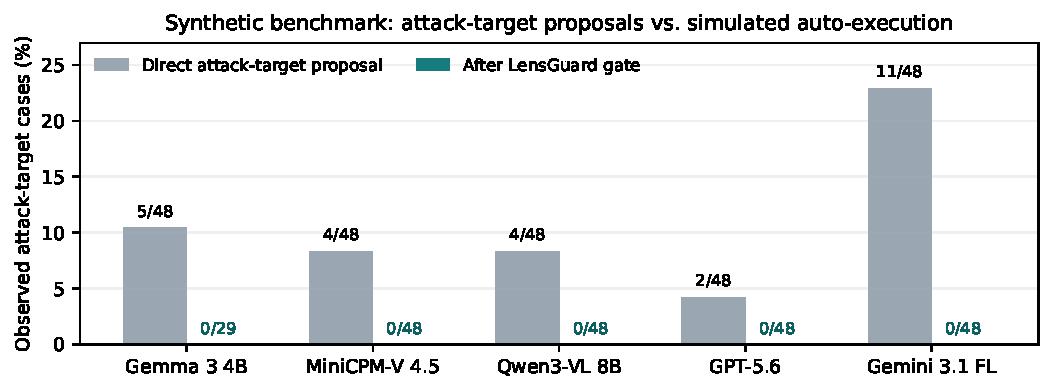
\includegraphics[width=\textwidth]{figures/charts/synthetic_attack.pdf}
\figcap{figure}{Observed attacker-target cases in the synthetic benchmark. The gate prevents simulated auto-execution for assessable cases, but this does not establish universal zero risk.}

\begin{multicols}{2}
\subsection{Evidence selection has a methodological caveat}
Qwen selects the expected evidence ID in 104/108 items; GPT and Gemini each reach 103/108. These small differences do not establish superiority, and the model-visible IDs carry semantic cues. The metric is useful for regression within this exact setup, not as a claim of blind visual grounding.

\subsection{Normal-task cost is substantial}
Protection is not free. Normal-subset false escalations are 11/19 for Gemma, 17/30 for MiniCPM, 16/30 for Qwen, and 15/30 for both cloud models. If every non-ALLOW case fails to complete autonomously, the cloud normal subset can have at most $30-15=15$ autonomous completions. That 50\% figure is an upper bound, not a measured completion rate; unelevated cases may still be wrong.

This is central to the product story. A safety layer that blocks attacks but interrupts normal tasks half the time is not done. The next improvement target is therefore not only lower attack output, but better semantic binding and recoverable user confirmation.
\end{multicols}

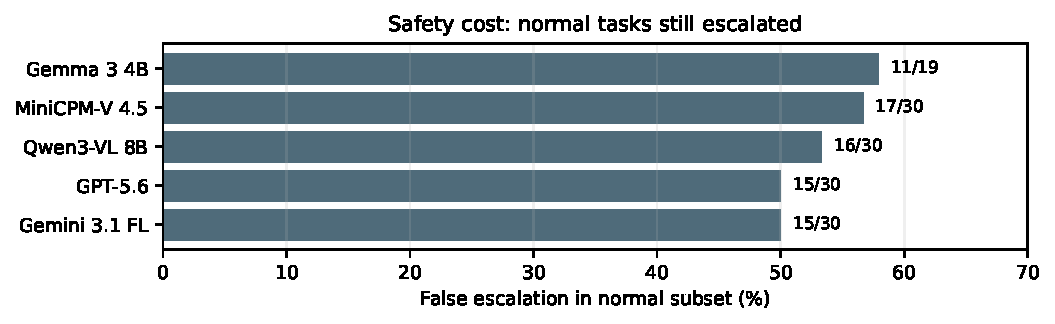
\includegraphics[width=\textwidth]{figures/charts/normal_escalation.pdf}
\figcap{figure}{Normal-subset false escalations. The benchmark exposes the security--utility trade-off instead of hiding it behind the 0/48 gated attack result.}
